\section{1174084 - Muhammad Reza Syachrani}
\subsection{Teori}
\begin{enumerate}
	\item Definisi Sejarah dan Perkembangan Kecerdasan Buatan
	\hfill\break
	Definisi Kecerdasan Buatan, Kecerdasan Buatan biasa disebut dengan istilah AI (Artificial Intelligence). AI merupakan tentang bagaimana cara untuk melengkapi sebuah komputer dengan kemampuan yang dimiliki oleh manusia. Dengan demikian, Diharapkan komputer mampu mengambil keputusan sendiri untuk berbagai kasus yang ditemuinya kemudian itulah yang disebut dengan kecerdasan buatan.  Kecerdasan buatan adalah kemampuan komputer yang dikendalikan konputer untuk melakukan tugas yang umumnya dikaitkan dengan sesuatu yang cerdas.
	\hfill\break
	Sejarah Kecerdasan Buatan, Kecerdasan buatan / Artificial intelligence mulai terbentuk pada tahun 1940 dan 1950. Pada awal 50-an, studi tentang “mesin berpikir” memiliki berbagai nama seperti cybernetics, teori automata, dan pemrosesan innformasi. Pada tahun 1956, para ilmuan jenius seperti Alan Turing, Norbert, Wiener, Claude Shannon dan Warren McCullough telah bekerja secara independen dibidang cybernetics, matematika, algoritma dan teori jaringan. Namun, seprang ilmuan komputer dan kognitif John McCarthy adalah orang yang dating dengan ide untuk bergabung dengan upaya penelitian terpisah ini kedalam satu bidang yang akan mempelajari topic baru untuk imajinasi manusia yaitu kecerdasan buatan.
    Pada tahun 1956, McCarthy yang sama mendirikan Konferensi Dartmouth di Hanover, New Hampshire. Tujuan dari bidang penelitian yang baru dibuat adalah untuk mengembangkan mesin yang dapat mensimulasikan setiap aspek kecerdasab. Oleh karena itu Konferensi Dartmouth 1956 dianggap sebagai kelahiran Kecerdasan Buatan.
    \hfill\break
    Perkembangan Kecerdasan Buatan, perkembangan kecerdasan buatan dapat menggantikan berbagai pekerjaan manusia seperti kasir, operator telepon, pengendara truk, dan lainnya. AI Summer 1 (1956-1973) Konferensi Dartmounth diikuti oleh 17 tahun kemajuan luar biasa. Proyek penelitian yang dilakukan di MIT, universitas di Edinburgh, Stanford dan Carnegie Mellon menerima dana besar-besaran, yang akhirnya membuahkan hasil. Selama tahun-tahun itulah komputer pemrograman mulai melakukan masalah aljabar, membuktikan teorema geometris, memahami dan menggunakan sintaks dan tata bahasa Inggris. Terlepas dari ditinggalkannya koneksionisme dan terjemahan mesin yang gagal, yang menunda penelitian Natural Language Processing (NLP) selama bertahun-tahun, banyak prestasi dari masa lalu yang membuat sejarah. Berikut ini beberapa diantaranya : Pelopor pembelajaran mesin, Ray Solomonoff dasar-dasar teori metematika AI, memperkenalkan metode Bayesian universal untuk inferensi dan preddiksi induktif Thomas Evans menciptakan program ANALOGI heuristik, yang memungkinkan komputer memecahkan masalah geometrianalogi Unimation, perusahaan robotika pertma didunia, menciptakan robot industri Unimate, yang bekerja pada jalur perakitan modil Genenral Motors. Joseph Weizenbaum membangun ELIZA-program interaktif yang dapat membawa percakapan dalam bahasan Inggris tentang topik apapun. Ross Quillian menunjukkan jaring semanik, sedangkan Jaime Carbonell (Sr.) mengembangkan Cendikia-program interaktif untuk instruksi yang dibantu komputer berdasarkan jaring semantik. Edward Feigenbaum dan Julian Feldman menerbitkan Computeks and Thought, kumpulan artikel pertama tentang AI.
	\item Definisi Supervised learning, klasifikasi, regresi, unsupervised learning, dataset, training set dan testing set.
	\hfill\break
	\begin{itemize}
		\item Supervised Learning
		\hfill\break
		Supervised Learning merupakan tugas pengumpulan data untuk menyimpulkan fungsi dari data pelatihan berlabel. Data pelatihan terdiri dari serangkaian contoh pelatihan. Dalam supervised learning, setiap contoh adalah pasangan yang terdiri dari objek input (biasanya vektor) dan nilai output yang diinginkan(juga disebut sinyal pengawasan super).
		\item Klasifikasi
		\hfill\break
		Klasifikasi adalah pembagian sesuatu menurut kelas-kelas.  Klasifikasi merupakan proses dari pengelompokkan benda berdasarkan ciri-ciri persamaan dan juga perbedaan. Dalam masalah klasifikasi, kami mencoba memprediksi sejumlah nilai terpisah.
		\item Regresi
		\hfill\break
		Regresi adalah metode analisis statistik yang digunakan untuk melihat pengaruh antara dua ataupun lebih variabel. Regresi adalah membahas masalah ketika variabel output adalah nilai riil atau berkelanjutan, seperti ”gaji” atau ”berat”.
		\item Unsupervised learning 
		\hfill\break
		Unsupervised Learning adalah pelatihan algoritma kecerdasan buatan (AI) menggunakan informasi yang tidak diklasifikasikan atau diberi label dan memungkinkan algoritma untuk bertindak atas informasi tersebut tanpa bimbingan. Dalam Unsupervised Learning, sistem AI dapat mengelompokkan informasi yang tidak disortir berdasarkan persamaan dan perbedaan meskipun tidak ada kategori yang disediakan.
		\item Data set
		\hfill\break
		Data set objek yang merepresentasikan data dan relasinya di memory. Strukturnya mirip dengan data di database. Dataset berisi koleksi dari datatable dan datarelation.
		\item Training Set
		\hfill\break
		Training Set adalah set digunakan oleh algoritma klassifikasi. Dapat dicontohkan dengan decision tree, bayesian, neural network dll. Semuanya dapat digunakan untuk membentuk sebuah model classifier
		\item Testing Set
		\hfill\break
		Testing Set merupakan set yang digunakan untuk mengukur sejauh mana classifier berhasil melakukan klasifikasi dengan benar. Dapat berfungsi sebagai meterai persetujuan, dan Anda tidak menggunakannya sampai akhir.
	\end{itemize}
\end{enumerate}
\subsection{Praktek}
\begin{enumerate}
	\item Instalasi Library scikit dari ianaconda, mencoba kompilasi dan uji coba ambil contoh kode dan lihat variabel explorer
	\hfill\break
	\begin{figure}[H]
		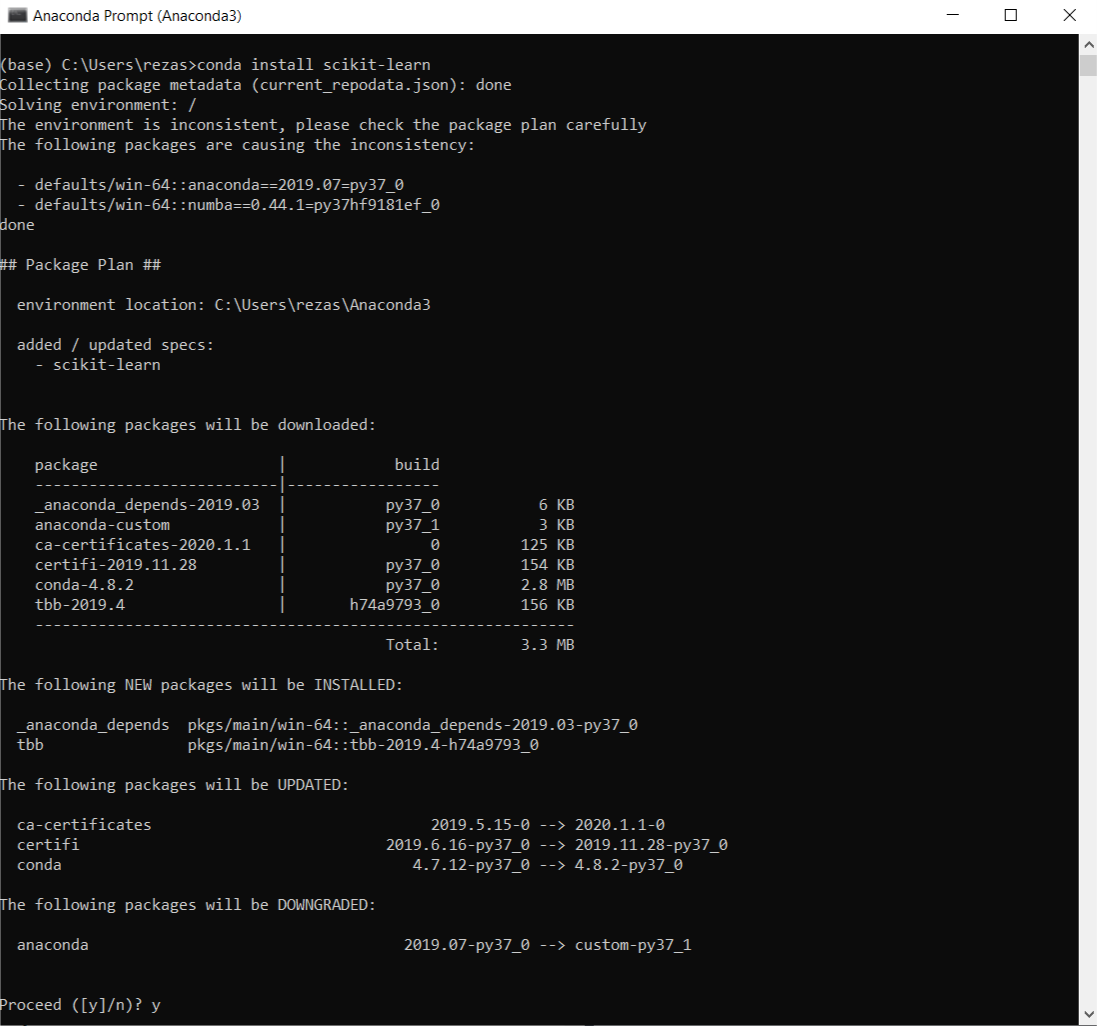
\includegraphics[width=4cm]{figures/1174084/1/1.png}
		\centering
		\caption{Instalasi Package Scikit Learn}
	\end{figure}
	\begin{figure}[H]
		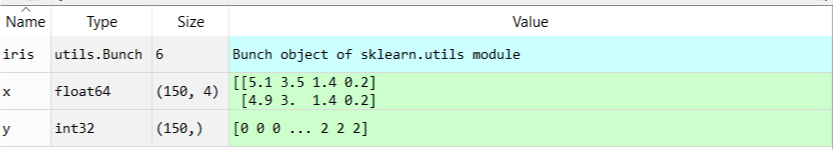
\includegraphics[width=4cm]{figures/1174084/1/2.png}
		\centering
		\caption{Isi Variabel Explorer}
	\end{figure}
	\item Mencoba loading an example dataset
	\hfill\break
	\lstinputlisting[firstline=7, lastline=11]{src/1174084/1/1174084.py}
	\item Mencoba Learning dan predicting
	\hfill\break
	\lstinputlisting[firstline=12, lastline=22]{src/1174084/1/1174084.py}
	\item Mencoba Model Persistence
	\hfill\break
	\lstinputlisting[firstline=23, lastline=33]{src/1174084/1/1174084.py}
	\item Mencoba Conventions
	\hfill\break
	\lstinputlisting[firstline=34, lastline=46]{src/1174084/1/1174084.py}
\end{enumerate}
\subsection{Penanganan Error}
\begin{enumerate}
	\item ScreenShoot Error
	\begin{figure}[H]
		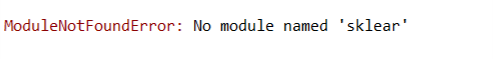
\includegraphics[width=4cm]{figures/1174084/1/error/1.png}
		\centering
		\caption{Module Error}
	\end{figure}
	\item Tuliskan Kode Error dan Jenis Error
	\begin{itemize}
		\item Module Error
	\end{itemize}
	\item Cara Penangan Error
	\begin{itemize}
		\item Module Error
		\hfill\break
		Dengan memperbaiki penulisan atau kesalahan dalam kode atau melakukan install package atau modul yang belum terinstal 
	\end{itemize}
\end{enumerate}
\subsection{Bukti Tidak Plagiat}
\begin{figure}[H]
	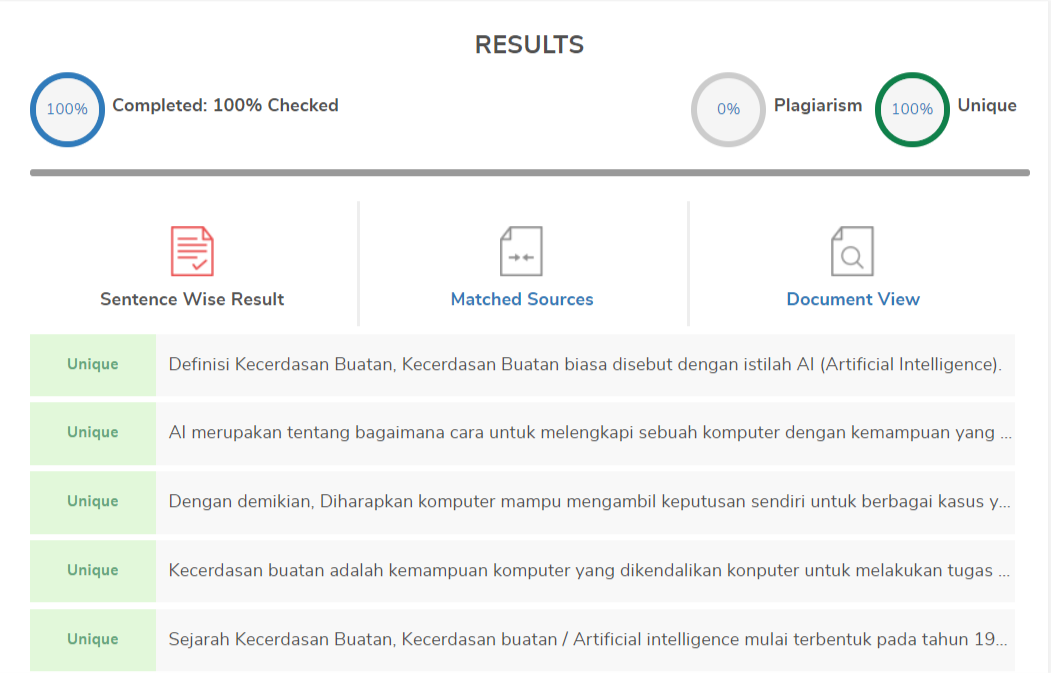
\includegraphics[width=4cm]{figures/1174084/1/plagiarisme.png}
	\centering
	\caption{Bukti Tidak Melakukan Plagiat}
\end{figure}